\chapter{Introduction}

\section{Purpose}


The \textit{Students\&Companies (S\&C)} platform bridges the gap between university students seeking
internships and companies offering them. It simplifies the process of matching students with internship
opportunities based on their skills, experiences, and preferences, as well as companies' requirements
and offered benefits.

The software involves three main actors: \textbf{students}, \textbf{companies}, and \textbf{universities}.

\begin{itemize}
    \item \textbf{Students} use the platform to search and apply for internships, submit their CVs, and
    receive recommendations tailored to their profiles.
    \item \textbf{Companies} advertise internships, specify requirements, and manage the selection
    process for suitable candidates.
    \item \textbf{Universities} monitor the execution of internships and handle complaints or
    issues that may arise.
\end{itemize}

S\&C features a \textbf{recommendation system} that matches students and internships using mechanisms
ranging from keyword-based searches to advanced statistical analyses. The platform also facilitates
communication, supports the selection process, and tracks internship progress to ensure transparency
for all involved parties.

\newpage
\section{Scope}

The Students\&Companies (S\&C) platform is a web application designed to facilitate communication and
matchmaking between university students seeking internships and companies offering them. The platform
simplifies and automates the process by enabling students to explore and apply for internships, while
also allowing companies to advertise their openings and identify suitable candidates. Additionally,
a sophisticated recommendation system enhances the user experience by automatically suggesting relevant
matches to both students and companies based on their preferences and requirements.

This document aims to outline the key architectural decisions behind the design and implementation of
the S\&C platform. Given the diverse user base, which includes students, companies, and universities,
and the need for simultaneous interaction among these parties, a web application was chosen as the
foundation. Its accessibility and ease of use ensure a seamless experience for users across various
locations and devices.

The complexity of the platform, along with the distinct functionalities it provides—such as recommendations,
selection processes, and feedback collection—led to the choice of a microservices architecture.
This architectural style was selected due to its ability to offer scalability, flexibility, resilience,
and modularity. Each microservice operates independently, allowing for targeted scaling based on
demand, individual updates and deployments, and clear separation of responsibilities.
The result is a system that is both maintainable and adaptable to evolving requirements.

From a deployment perspective, the system adopts a three-tier architecture. The user client
layer represents the web and mobile interfaces used by students, companies, and universities.
The server layer hosts all microservices, which manage the business logic and application
functionality. Finally, the shared database layer ensures consistency in data storage,
maintaining information about users, internships, recommendations, and feedback.

To manage interactions between microservices, the platform uses a combination of communication
patterns based on specific functional needs. For real-time or asynchronous interactions, an
event-driven communication model is employed. In this approach, some microservices act as event
publishers while others function as consumers. For example, the Notification Microservice processes
events related to complaints, messages, and new recommendations, while other services publish events
to reflect changes in system states, such as the pubblication of a new message on the communication platform
or the acceptance of a student for an interview.
 
For functionalities that do not require immediate interactions, synchronous communication mechanisms
are used. This includes scenarios such as retrieving a list of internships or submitting CVs, where
sequential processing and immediate feedback are necessary. The combination of event-driven and
synchronous communication ensures that the system remains both responsive and straightforward to
use, catering to the dynamic needs of its users.

All these architectural choices are just mentioned here to provide an overview of the system; they
will be better explained and unpacked down the line of this document. The following image shows
the major components of the Students\&Companies system.
\newline
\newline

\begin{figure} [H]
    \centering
    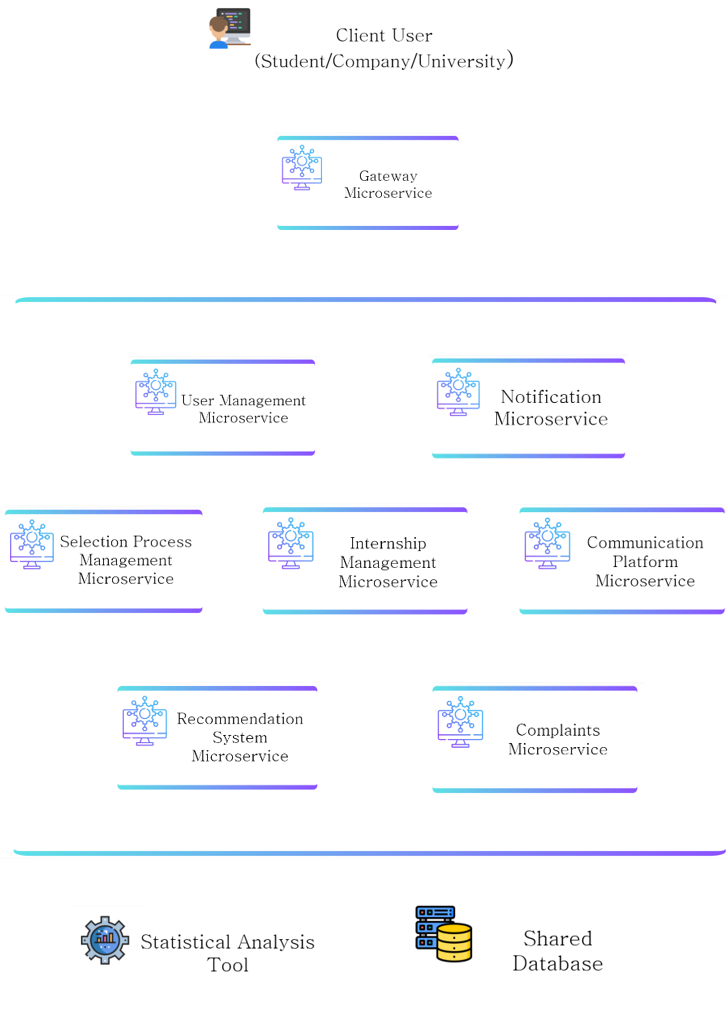
\includegraphics [width=0.75\linewidth] {MicroservicesImage.png}
\end{figure}


\newpage
\section{Definitions, Acronyms, Abbreviations}
\subsection{Definitions}
\subsection{Acronyms}
\subsection{Abbreviations}

\newpage
\section{Reference Documents}

\newpage
\section{Document Structure}